\section{Exploración de la tasa de mutación}

\begin{figure}[]
	\centering	
	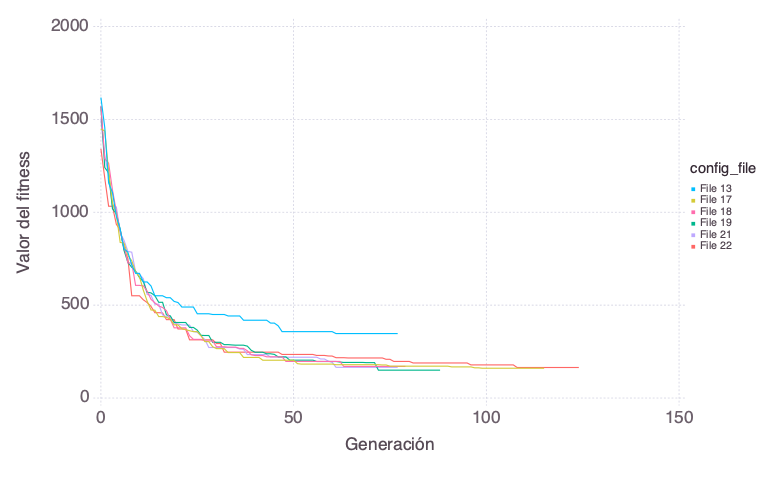
\includegraphics[scale=0.5]{../data/Plots/mutation_rate_executions.png}
	\caption{ Variación del valor del fitness a lo largo de las generaciones para los ficheros con mejor valor para cada fichero de configuración, variando la tasa de mutación}
    \label{fig:tasa_mutacion_variacion_generacion}
\end{figure}

Para explorar el comportamiento del algoritmo al cambiar la tasa de mutación se han usado los ficheros del 15 al 23, ver presentes en el Anexo \ref{subsect:config_file}. En la
Tabla \ref{tab:exploracion_tasa_mutacion} solo se han añadido los que presentan diferencia con la configuración 13. En esta tabla se puede ver que cambiando la tasa de mutación
de las castas se obtienen valores objetivamente mejores. Por ejemplo, el caso de la configuración 19 [\ref{subsect:config_file_19}], a pesar de tener la mayor desviación estándar,
es decir, teniendo la mayor dispersión de valores, es la que tiene mejor mediana de valor de la función del fitness. En la Figura \ref{fig:tasa_mutacion_variacion_generacion} se puede 
ver como los ficheros en los que se ha cambiado las tasas de mutación, además de durar más generaciones debido a que mantiene la diversidad durante más tiempo, obtiene
valores más pequeños de fitness.


\begin{table}[]
    \centering
    \begin{tabular}{|c|c|c|c|c|c|}
    \hline
    \textbf{Config.} & \textbf{\begin{tabular}[c]{@{}c@{}}Tasa\\ de\\ mutación\end{tabular}}                                & \textbf{\begin{tabular}[c]{@{}c@{}}Mediana \\ mejor valor \\ de fitness\end{tabular}} & \textbf{\begin{tabular}[c]{@{}c@{}}Mediana \\ \# ejecuciones \\ de f\end{tabular}} & \textbf{\begin{tabular}[c]{@{}c@{}}$\sigma$\\ mejor valor\\ de fitness\end{tabular}} & \textbf{\begin{tabular}[c]{@{}c@{}}$\sigma$\\ \# ejecuciones \\ de f\end{tabular}} \\ \hline
    13 [\ref{subsect:config_file_13}]  & \begin{tabular}[c]{@{}c@{}}ALFA:10\\ BETA: 10\\ GAMMA: 10\\ DELTA: 10\\ EPSILON: 10\end{tabular}     & 367.07                                                                                & 512473.0                                                                           & 23.38                                                                         & 124996.18                                                                   \\ \hline
    17 [\ref{subsect:config_file_17}]  & \begin{tabular}[c]{@{}c@{}}ALFA: 5\\ BETA: 10\\ GAMMA: 15\\ DELTA: 20\\ EPSILON: 25\end{tabular}     & 174.16                                                                                & 666019.0                                                                           & 17.27                                                                         & 139365.89                                                                   \\ \hline
    18 [\ref{subsect:config_file_18}]  & \begin{tabular}[c]{@{}c@{}}ALFA: 5\\ BETA: 10\\ GAMMA: 20\\ DELTA: 25\\ EPSILON: 30\end{tabular}     & 193.71                                                                                & 648559.0                                                                           & 15.20                                                                         & 78935.72                                                                    \\ \hline
    19 [\ref{subsect:config_file_19}]  & \begin{tabular}[c]{@{}c@{}}ALFA: 5\\ BETA: 10\\ GAMMA: 25\\ DELTA: 30\\ EPSILON: 40\end{tabular}     & 186.31                                                                                & 655014.0                                                                           & 26.32                                                                         & 116351.11                                                                   \\ \hline
    21 [\ref{subsect:config_file_20}]  & \begin{tabular}[c]{@{}c@{}}ALFA: 5\\ BETA: 10\\ GAMMA: 30\\ DELTA: 35\\ EPSILON: 45\end{tabular}     & 211.39                                                                                & 639449.0                                                                           & 21.16                                                                         & 144132.16                                                                   \\ \hline
    22 [\ref{subsect:config_file_21}]  & \begin{tabular}[c]{@{}c@{}}ALFA: 5\\ BETA: 10\\ GAMMA: 30\\ DELTA: 40\\ EPSILON: 50\end{tabular}     & 190.76                                                                                & 646056.0                                                                           & 22.19                                                                         & 120232.35                                                                   \\ \hline
    \end{tabular}
    \caption{Resultados exploración del tamaño del cromosoma, variando la tasa de mutación}
    \label{tab:exploracion_tasa_mutacion}
\end{table}
